\section{The Model Context Protocol}
\label{sec:mcp}

The recap showed that in \msa{} every check on a tool call runs inside the harness, in the agent's
own process (\cref{sec:recap}). A check that runs inside the agent's own process can be switched off
or avoided, and the rest of this lecture studies that limitation from the attacker's side. This section first explains the limitation, then introduces the
Model Context Protocol (MCP), which moves tools into separate programs and divides the work of a
tool call among a host, its clients and its servers. We follow one tool call through the protocol and
ask which component performs each of Lecture~4's five operations: find, bind, check, run and
observe.

\subsection{Checks inside the agent's process}
\label{sec:mcp-inside}

A rule enforced inside the agent's own process can be disabled or bypassed by the agent. The
limitation matters because the guarantees of a tool call rest on such rules. They come from the tool
contract and from the harness. None of them comes from the model.

The guarantees of Lecture~4 (\cref{tab:recap-guarantees}) include that only registered tools run,
that the arguments match the tool's parameters, and that writes stay inside the workspace. The model
only proposes a call. Code that the harness runs after the model has replied decides whether the
call is allowed, whether its arguments fit and where it may write.

A process is a running program, to which the operating system gives its own memory and the
permissions of the user who started it. In \msa{}, the agent's own code shares one process and one
set of permissions with the dispatcher. Every check between them, such as the path check that keeps
writes inside the workspace, runs in that process too.

Code that runs in a process can do whatever the process is permitted to do. It can change the
settings that switch a check on. It can also reach a file by a route that never passes through the
check.

Code actions, introduced in Lecture~4, take the second route. A code action is an action written as
a program that the harness runs in an interpreter, and the program executes with every right of the
harness process. A program that writes a file directly never calls \demoref{edit}. None of the
dispatcher's checks applies to it, and the path check inside \demoref{edit} never runs.

An agent misled by text in its inputs, or an attacker who reaches its settings, can take either
route. OpenClaw, an open-source personal AI assistant, is the case study that closes this lecture.
In both documented attacks on it, an attacker who reached the agent's settings or its inputs switched
off or got past a control that lived inside the agent's own process and configuration
(\cref{sec:openclaw}).

MITRE ATLAS, a catalog of adversary techniques against AI-enabled systems (\cref{sec:threats}),
records the techniques by which such rules are disabled or bypassed. Lecture~6 studies enforcement
outside the agent with NVIDIA OpenShell, a system that moves enforcement to the operating-system
kernel and to a separate supervising process that the agent cannot reach.

Before studying attacks, we study the protocol through which an agent reaches tools that run outside
its harness. When a tool moves into another program, the dispatcher's checks are divided among
several components. For each rule, we must then ask which component enforces it.

\subsection{What MCP standardizes}
\label{sec:mcp-what}

MCP is an open standard for connecting AI applications to external systems. Through MCP, an
application connects to data sources such as local files and databases, to tools such as search
engines and calculators, and to workflows such as specialized prompts. Lecture~4 introduced MCP
briefly as a response to the $N \times M$ integration problem. This section and
\cref{sec:mcpcontract} study the protocol itself, in revision 2026-07-28 of its specification.
\Cref{def:mcp} defines MCP by comparison with a familiar connector.

\begin{definition}[Model Context Protocol]
\label{def:mcp}
``MCP (Model Context Protocol) is an open-source standard for connecting AI applications to external
systems. [\ldots] Think of MCP like a USB-C port for AI applications. Just as USB-C provides a
standardized way to connect electronic devices, MCP provides a standardized way to connect AI
applications to external systems.'' \citep{mcp-intro}
\end{definition}

The comparison describes one standard port in place of a different cable for every device. An
application that implements MCP can use any MCP server, and a tool offered through an MCP server
works with any application that implements MCP. The applications that support MCP include Claude,
ChatGPT, Visual Studio Code and Cursor. Anthropic introduced the protocol in November 2024
\citep{anthropic2024mcp}.

MCP is the shared protocol that reduces the $N \times M$ integrations of the recap to $N + M$. Each
application implements the protocol once, and each tool is offered once, through a server.

The name states what the protocol standardizes. A model's context, as Lecture~2 defined it, is the
input that the model receives in one call. MCP standardizes how an application brings into that
input the data and the actions that external systems offer. MCP provides ``a standardized way to
connect LLMs with the context they need'' \citep{mcp-spec-2026}.

\subsection{Tools, resources and prompts}
\label{sec:mcp-features}

An MCP server offers tools, resources and prompts \citep{mcp-spec-2026}. A tool is a function that
the model can ask to execute. It is the tool of Lecture~2: an action that the agent requests by
name, with arguments, and that another program carries out. A \textbf{resource} is data that a server makes
available for the user or the model to use, such as the text of a file. An \textbf{MCP prompt} is a
templated message or workflow that a server offers to users. We add ``MCP'' to its name because
``prompt'' alone could mean the model's input. \Cref{tab:mcp-features} gives one example of each
from our running task.

\begin{table}[htbp]
  \caption{The features that an MCP server can offer, with an example of each from the running
  task.}
  \label{tab:mcp-features}
  \begin{adjustbox}{width=\linewidth}\begin{tabularx}{\linewidth}{L{0.2\linewidth}XL{0.3\linewidth}}
    \toprule
    \textbf{Feature} & \textbf{What it is} & \textbf{Example} \\
    \midrule
    \textbf{Tool} & A function for the model to execute & \demoref{edit(path, old, new)} \\
    \textbf{Resource} & Data for the user or the model to use & The text of \demoref{src/parse.py} \\
    \textbf{MCP prompt} & A templated message or workflow for users & A template that asks for a review of a change \\
    \bottomrule
  \end{tabularx}\end{adjustbox}
\end{table}

This lecture uses only tools, because tools are the features through which a model acts on the
world. Resources and MCP prompts travel over the same connection as tools and in the same message
format.

A server states which features it offers by declaring capabilities. A \textbf{capability} is a
feature that a server declares it supports, so that a client knows what it can ask for. A server that
offers tools, for example, must declare the tools capability. A client therefore learns from the
server itself whether to ask it for tools, resources or MCP prompts. It asks the server through
\demoref{server/discover}, a request that \cref{sec:mcp-methods} describes.

\subsection{One request from the user to the server}
\label{sec:mcp-request}

A request from a user crosses several components, and MCP covers the exchange between two of them,
the MCP client and the MCP server. Each exchange between two neighboring components is a
\textbf{hop}, and each hop can follow its own standard. \Cref{fig:mcp-request} follows a request in the constructed example of Lecture~4. The user asks an
AI application to fix an off-by-one error in \demoref{src/parse.py}, and an MCP server offers the
\demoref{edit} tool. The numbers in the figure mark the following steps:
\be
\item The user asks the application to fix the off-by-one error.
\item The application sends the question to the model, together with the list of tools that its
servers offer, written in the model vendor's native format.
\item The model replies with a call to \demoref{edit}.
\item The application's MCP client sends the edit request to the MCP server, and later receives
the result.
\item Before it returns the result, the server changes the file.
\item The application returns the model's answer to the user.
\ee

\begin{figure*}[tb]
  \centering
  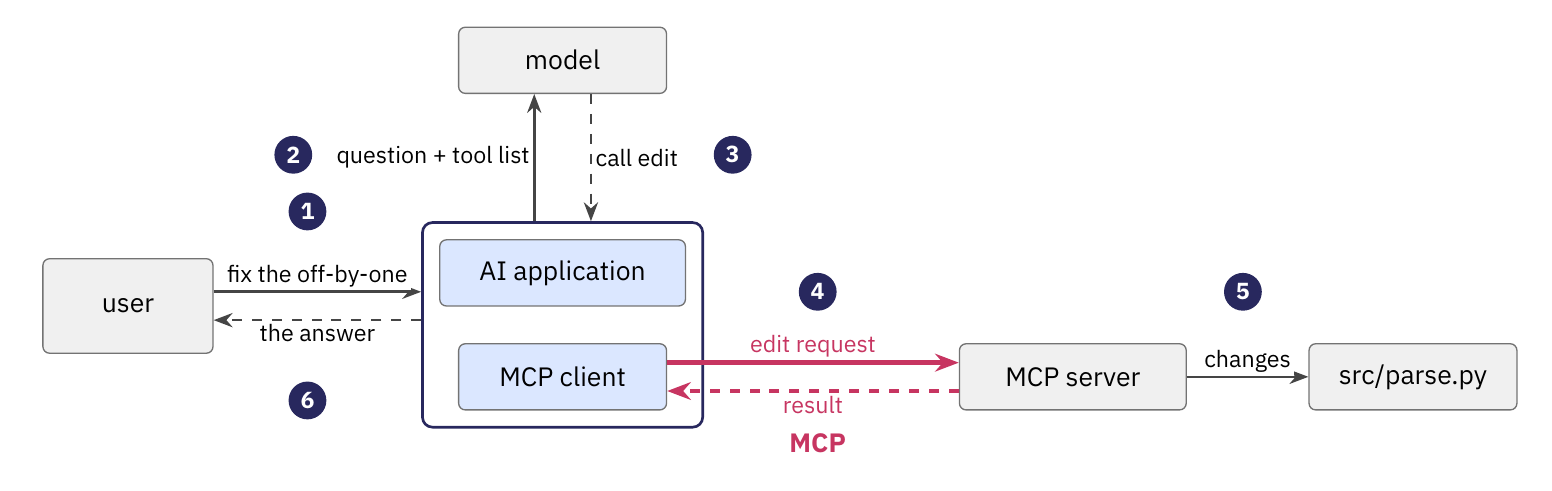
\includegraphics[width=\textwidth]{figures/deck/499fa33904.png}
  \caption{One request in an application that uses MCP, with steps numbered as in the text. Only
  the hop between the MCP client and the MCP server, drawn in color, uses MCP. The hop to the model
  uses the vendor's native tool calling.}
  \label{fig:mcp-request}
\end{figure*}

The hop to the model, steps 2 and 3, uses the native tool calling of Lecture~4, in which the request
to the model API lists the tools and the reply returns each tool call in a structured field. An
application that uses MCP therefore still uses native tool calling. The MCP components of the
request are the server, the client, and the application that contains the client, which MCP calls
the host.

\subsection{The server}
\label{sec:mcp-server}

An MCP \textbf{server} is a separate program, written once by the owner of a tool, that offers
tools, resources and MCP prompts \citep{mcp-spec-2026}. Any application that implements MCP can
use it, so servers are the $M$ side of the $N + M$ count. The term keeps its meaning from
Lecture~4, where a server is a separate program that offers tools and runs them. The MCP project
maintains reference servers, among them a Filesystem server and a Git server \citep{mcp-servers},
and companies publish official servers for their own products.

A server runs as a separate process. It is either a subprocess that the application starts on the
same machine, or a service that the application reaches over HTTP, on another machine or on the
user's own machine. The mechanism that carries messages between a client and a server is the
transport, a term that keeps its meaning from Lecture~4. MCP defines stdio and
Streamable HTTP as its standard transports:
\bi
\item \textbf{stdio.} The application starts the server as a subprocess, and the two exchange
messages over the subprocess's standard streams. The client writes each message to the server's
standard input and reads the replies from its standard output, one message per line.
\item \textbf{Streamable HTTP.} The server runs as a web service, and the client sends each message
as one HTTP POST request to a single address on the server, its endpoint. This transport suits a
server on another machine.
\ei
\Cref{sec:mcpcontract} describes how each transport marks where a message ends and how a reply can
stream.

Our illustrative edit server moves the course's \demoref{edit} tool into an MCP server written with
the official Python SDK \citep{mcp-python-sdk}. An SDK (software development kit) is a library that
implements the protocol, so that the server's author writes only the tool. \Cref{lst:mcp-server}
shows the server in outline.

\noindent\begin{minipage}{\linewidth}
\begin{lstlisting}[basicstyle=\ttfamily\footnotesize, caption={Illustrative code for the edit server, written with the official Python SDK.}, label=lst:mcp-server]
from typing import TypedDict
from mcp.server import MCPServer

mcp = MCPServer("workspace")

class EditResult(TypedDict):
    path: str
    replaced: int

@mcp.tool()
def edit(path: str, old: str, new: str) -> EditResult:
    """Replace one exact occurrence of old with new."""
    ...
\end{lstlisting}
\end{minipage}

The listing has the following parts:
\bi
\item \textbf{The server object.} \demoref{MCPServer("workspace")} creates a server named
\demoref{workspace}.
\item \textbf{The result type.} \demoref{EditResult} names the fields of a successful result: the
path of the edited file and the number of replacements made.
\item \textbf{The decorator.} \demoref{@mcp.tool()} registers the function as a tool of the server,
much as Lecture~4's registry maps a tool's name to its function.
\item \textbf{The function.} Its body, elided here, is the course's \demoref{edit} tool. The server
holds its workspace and refuses any path outside it.
\ei

From the decorated function, the SDK derives the tool definition, the part of the tool contract that
the model receives (\cref{sec:recap}). It takes the name from the function's name, the description from its
docstring, and the input schema from the type hints of its parameters. The \textbf{input schema} (\demoref{inputSchema}) is MCP's name for Lecture~4's argument
schema. It is a JSON Schema, a description in a standard language of the shape that JSON data must
have, and it gives the names and types of the arguments and says which are required. The server's
author writes no schema by hand. \Cref{sec:mcpcontract} shows the whole definition that the SDK
generates. It also includes an output schema, a JSON Schema that the data in the tool's result must
match, which the SDK derives from \demoref{EditResult}.

\subsection{The host and its clients}
\label{sec:mcp-host}

The application that the user runs is the \textbf{host}. It may be a chat application such as
Claude Desktop, an IDE or an agent harness. A harness like ours, built with LangGraph
\citep{langchain-tools}, takes the host role when it connects to MCP servers. Product documentation
often calls the whole application the client. In MCP's terms, the application is the host, and a
client is one of its components.

For each server, the host creates one \textbf{client}, a component that starts or connects to that
server and sends it requests. The relation is one to one: each client communicates with exactly one
server. In code, a client is an object that holds the connection to one server. Lecture~4 called the
client the part of the harness that exchanges messages with a server. When a harness like ours takes
the host role, its clients are that part.

Claude Desktop, for example, reads a list of servers from its configuration and starts each listed
server whenever it launches \citep{mcp-connect-local}. With the official Python SDK, the host's code
opens a client on a server and calls a tool by its name with a dictionary of arguments
\citep{mcp-python-sdk}. Each such call sends one request to the server.

\begin{figure*}[tb]
  \centering
  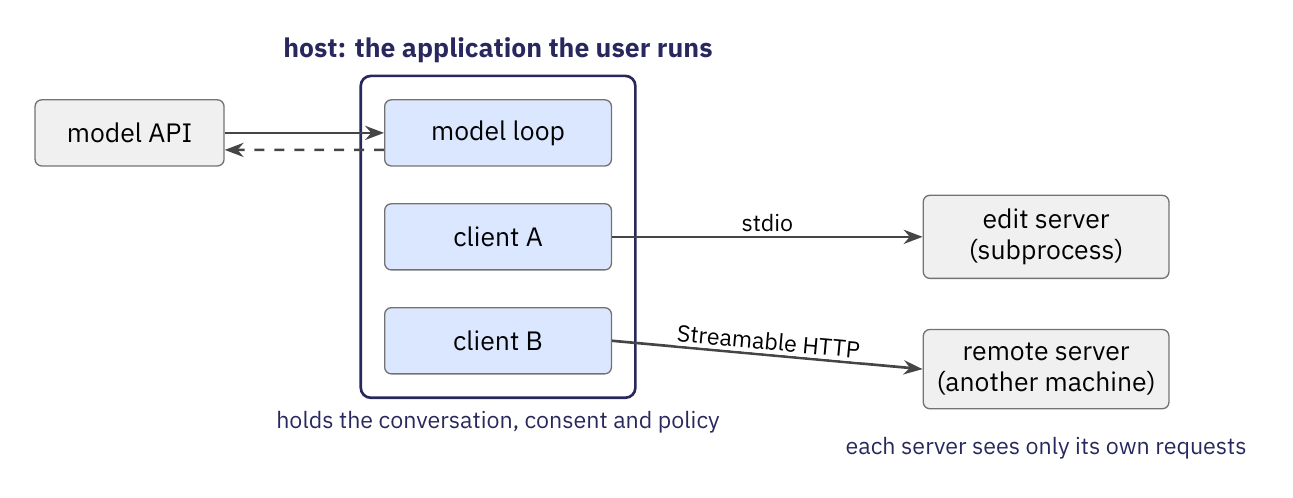
\includegraphics[width=0.75\textwidth]{figures/deck/eb08723398.png}
  \caption{A host with two clients. Client A runs the edit server as a subprocess over stdio, and
  client B reaches a remote server over Streamable HTTP. The host holds the conversation, the
  user's consent and the policy, and each server sees only its own requests.}
  \label{fig:mcp-connections}
\end{figure*}

\Cref{fig:mcp-connections} shows a host with two clients. Client A starts the illustrative edit
server as a subprocess and talks to it over stdio. Client B reaches a remote server on another
machine over Streamable HTTP. The host's model loop exchanges messages with the model API. The host
coordinates its clients and holds what they share:
\bi
\item \textbf{Clients.} The host creates and manages its clients, one for each server.
\item \textbf{Conversation.} The host keeps the full conversation and combines the context gathered
through all its clients.
\item \textbf{Policy and consent.} The host enforces security policies and consent requirements,
and it handles the user's decisions about what to authorize. Policy keeps its meaning from
Lecture~4: the rules that decide whether a requested call is allowed. \textbf{Consent} is the user's
approval, which the host obtains before it invokes a tool (\cref{sec:mcp-path}).
\ei

Servers are kept apart from the conversation and from each other. One design principle of MCP is
that ``servers should not be able to read the whole conversation, nor `see into' other servers'',
and that the full conversation history stays with the host \citep{mcp-spec-2026}. Each server
receives only the requests that its client sends, so it learns only what the host chooses to put in
them. The edit server sees edit requests and their arguments. It sees the user's other questions
only if the host puts them into a request. It does not see the traffic of the remote server, which
passes through another client. This matters because a server is written by the
tool's owner, who may be someone other than the author of the host, and the host need not trust it
with the whole conversation.

In Lecture~4, every operation of a tool call took place inside the harness's process. Under MCP, the
dispatcher's work is split: the host keeps the conversation and the policy, and the server runs the
tool.
\Cref{sec:mcp-operations} sets out the split operation by operation.

\subsection{Messages and methods}
\label{sec:mcp-methods}

Every MCP message is a \textbf{JSON-RPC} message \citep{mcp-spec-2026}. JSON-RPC is a standard
format, written in JSON, for remote procedure calls, the calls to a procedure in another process or
on another machine that Lecture~4 described. A JSON-RPC message is a request, a response or a
notification:
\bi
\item \textbf{Request.} A request names a \textbf{method}, the action it asks the receiver to
perform, such as \demoref{tools/call}. It carries a \textbf{request ID}, a string or an integer
chosen by the sender, and the method's parameters.
\item \textbf{Response.} A response repeats the request ID and carries either a result or an error.
The ID lets the sender match each reply to its request. A sender never reuses the ID of a request
that is still waiting for its response.
\item \textbf{Notification.} A \textbf{notification} names a method but carries no ID, and its
receiver sends no response.
\ei

MCP defines each kind of request as a method. \Cref{tab:mcp-methods} lists the methods that this
lecture uses and the party that sends each one. The client sends every request in the table. The
last row is a kind of result, which the server returns inside a reply when it needs more input from
the client.

\begin{table}[htbp]
  \caption{The MCP methods that this lecture uses, with the party that sends each one and its
  purpose.}
  \label{tab:mcp-methods}
  \begin{adjustbox}{width=\linewidth}\begin{tabularx}{\linewidth}{L{0.37\linewidth}L{0.15\linewidth}X}
    \toprule
    \textbf{Method} & \textbf{Sent by} & \textbf{Purpose} \\
    \midrule
    \demoref{server/discover} & Client & Returns the server's protocol versions, capabilities and identity. \\
    \demoref{tools/list}, \demoref{tools/call} & Client & List the server's tools, and call one of them. \\
    \demoref{resources/list}, \demoref{resources/read} & Client & List the server's resources, and read one. \\
    \demoref{prompts/list}, \demoref{prompts/get} & Client & List the server's MCP prompts, and fetch one. \\
    \demoref{completion/complete} & Client & Suggests completions for an argument's value. \\
    \demoref{subscriptions/listen} & Client & Opens one stream for the server's change notifications. \\
    An \demoref{input\_required} result & Server & Asks for more input. The client retries the request with that input. \\
    \bottomrule
  \end{tabularx}\end{adjustbox}
\end{table}

An \demoref{input\_required} result is the only entry in the table that the server sends. A server
sends responses and notifications, and it never sends a request of its own. When it needs more input
to finish a request, it returns a result of the type \demoref{input\_required}. The client then
sends the request again as a new request, with a new request ID, that carries the input the server
asked for.

What a server must support follows from its capabilities. A server implements only the features
that it declares as capabilities. Every server must also implement \demoref{server/discover},
which a client may call before any other request to learn the protocol versions that the server
supports, its capabilities and its identity. MCP defines a few further messages, such as the
progress notifications that a server sends before a result. \Cref{sec:mcpcontract} covers them,
together with the cancellation of a request.

A message names its method in its body, so both transports carry every method in the same way.
Over stdio, each message is one line of text. Over Streamable HTTP, each message from the client is
one POST to the server's single endpoint, and the server's messages return in the HTTP response.

\subsection{From MCP tools to native tool definitions}
\label{sec:mcp-native}

The host translates every MCP tool into the format of the model API, so no MCP message reaches the
model. It converts each tool that a server lists into a \textbf{native tool definition}, a tool
definition in Lecture~4's sense written in the format of one model vendor, and sends these
definitions to the model API. \Cref{lst:mcp-toolslist} shows the illustrative edit
server's answer to \demoref{tools/list}, shortened to the fields that the model needs.
\Cref{lst:mcp-convert} shows host code that converts each listed tool into the native format of
OpenAI's Chat Completions API.

\noindent\begin{minipage}{\linewidth}
\begin{lstlisting}[basicstyle=\ttfamily\footnotesize, caption={Illustrative answer of the edit server to \texttt{tools/list}, shortened to the fields that the model receives.}, label=lst:mcp-toolslist]
{"tools": [{
   "name": "edit",
   "description": "Replace one exact occurrence of old with new.",
   "inputSchema": {
     "type": "object",
     "properties": {"path": {"type": "string"},
                    "old":  {"type": "string"},
                    "new":  {"type": "string"}},
     "required": ["path", "old", "new"]}}]}
\end{lstlisting}
\end{minipage}

\noindent\begin{minipage}{\linewidth}
\begin{lstlisting}[basicstyle=\ttfamily\footnotesize, caption={Illustrative host code that builds one native tool definition for each listed tool.}, label=lst:mcp-convert]
tools = [{"type": "function",
          "function": {"name": t["name"],
                       "description": t["description"],
                       "parameters": t["inputSchema"]}}
         for t in listed["tools"]]
\end{lstlisting}
\end{minipage}

In \cref{lst:mcp-convert}, the variable \demoref{listed} holds the answer to \demoref{tools/list}.
Each native tool definition is an object whose \demoref{type} is \demoref{function} and whose
\demoref{function} field holds the tool's fields, as OpenAI's format requires. The conversion copies
three fields. The tool's \demoref{name} and \demoref{description} keep their
names, and the MCP field \demoref{inputSchema} becomes the vendor's \demoref{parameters}. For
Anthropic's API, the same schema becomes \demoref{input\_schema}. The model therefore receives the
name, the description and the input schema, which are the parts of Lecture~4's tool definition.

An MCP tool definition can carry more fields than the host passes to the model: a display title, an
output schema for the result's data, annotations that hint at the tool's side effects, icons, and a
\demoref{\_meta} field for further metadata (\cref{sec:mcpcontract}). The answer to \demoref{tools/list} also carries \demoref{ttlMs}, the time
in milliseconds for which the client may cache the list \citep{mcp-spec-2026}.

MCP messages travel both before and after the call to the model API. Before the call, the client
lists the server's tools. After the model has replied, the client sends the tool call to the server
and receives the result. Native tool calling covers the call to the model API itself. The two
standards therefore work together: each covers its own hop, and an application uses both. A server
written once can serve a model from any vendor, because the host translates its definitions into the
format that the vendor's API expects.

\subsection{The path of one tool call}
\label{sec:mcp-path}

\Cref{fig:mcp-path} follows one call of \demoref{edit} from the first listing of tools to the
model's next input. It draws a vertical line, called a lifeline, for each party: the model API, the
host, the client and the edit server. Time runs downward, and each arrow is a message between two
parties. The call takes these steps:
\be
\item \textbf{List.} The client sends \demoref{tools/list}, and the server returns its tool
definitions.
\item \textbf{Ask the model.} The host sends the model API the conversation's messages and the
native tool definitions.
\item \textbf{Receive the call.} The model API returns a tool call in the vendor's format.
\item \textbf{Map and approve.} The host maps the call to a server and a tool, and it obtains the
user's consent.
\item \textbf{Send.} The client sends \demoref{tools/call} with the tool's name and arguments.
\item \textbf{Validate and run.} The server validates the arguments and then runs \demoref{edit}.
\item \textbf{Return.} The result travels back through the client to the host, with its content and
its \demoref{isError} flag, which is true when the tool failed (\cref{sec:mcp-results}).
\item \textbf{Feed back.} The host adds the result to the messages of the next model call.
\ee

\begin{figure*}[tb]
  \centering
  \definecolor{mcpnavy}{HTML}{28285E}
  \begin{tikzpicture}[x=1cm, y=1cm,
      head/.style={minimum width=2.3cm},
      life/.style={draw=ibmfg!30},
      num/.style={circle, fill=mcpnavy, text=white, font=\sffamily\bfseries\footnotesize,
                  inner sep=0pt, minimum size=4.4mm},
      act/.style={draw=ibmfg!60, rounded corners=2pt, fill=black!6, font=\sffamily\footnotesize,
                  inner sep=2.5pt},
      msg/.style={font=\sffamily\footnotesize, above, inner sep=2pt, align=center},
      proc/.style={font=\sffamily\footnotesize, text=mcpnavy},
    ]
    \def\xm{0} \def\xh{5.8} \def\xc{9.8} \def\xs{14.4}
    \node[rnode, head] at (\xm,0) {model API};
    \node[mnode, head] at (\xh,0) {host};
    \node[mnode, head] at (\xc,0) {client};
    \node[rnode, head] at (\xs,0) {edit server};
    \foreach \x in {\xm,\xh,\xc,\xs} \draw[life] (\x,-0.4) -- (\x,-7.2);
    % 1: list the tools
    \draw[flow] (\xc,-1.0) -- node[msg] {\texttt{tools/list}} (\xs,-1.0);
    \draw[back] (\xs,-1.6) -- node[msg] {tool definitions} (\xc,-1.6);
    \node[num] at (-1.3,-1.3) {1};
    % 2: ask the model
    \draw[flow] (\xh,-2.5) -- node[msg] {messages + tool definitions\\(vendor format)} (\xm,-2.5);
    \node[num] at (-1.3,-2.5) {2};
    % 3: the model's tool call
    \draw[back] (\xm,-3.2) -- node[msg] {tool call (vendor format)} (\xh,-3.2);
    \node[num] at (-1.3,-3.2) {3};
    % 4: map and obtain consent
    \node[act] at (\xh,-3.9) {map to server, ask the user};
    \node[num] at (-1.3,-3.9) {4};
    % 5: tools/call
    \draw[flow] (\xh,-4.6) -- (\xc,-4.6);
    \draw[flow] (\xc,-4.6) -- node[msg] {\texttt{tools/call}: \texttt{edit}, arguments} (\xs,-4.6);
    \node[num] at (-1.3,-4.6) {5};
    % 6: validate, then run
    \node[act] at (\xs,-5.3) {validate, then run \texttt{edit}};
    \node[num] at (-1.3,-5.3) {6};
    % 7: the result returns
    \draw[back] (\xs,-6.0) -- node[msg] {result: content, \texttt{isError}} (\xc,-6.0);
    \draw[back] (\xc,-6.0) -- (\xh,-6.0);
    \node[num] at (-1.3,-6.0) {7};
    % 8: the result enters the next model call
    \draw[flow] (\xh,-6.7) -- node[msg] {messages + tool result} (\xm,-6.7);
    \node[num] at (-1.3,-6.7) {8};
    % processes
    \draw[mcpnavy] (\xh-0.4,-7.35) -- ++(0,-0.15) -- (\xc+0.4,-7.5) -- ++(0,0.15);
    \draw[mcpnavy] ({(\xh+\xc)/2},-7.5) -- ++(0,-0.1);
    \node[proc] at ({(\xh+\xc)/2},-7.85) {one process};
    \node[proc] at (\xs,-7.85) {a separate process};
  \end{tikzpicture}
  \caption{The path of one MCP tool call, with steps numbered as in the text. Steps 2, 3 and 8 use
  the model vendor's native format, and steps 1, 5 and 7 are MCP messages. The host and its client
  run in one process, and the server runs in another.}
  \label{fig:mcp-path}
\end{figure*}

The steps belong to different hops. Steps 1, 5 and 7 are MCP messages between the client and the
server. Steps 2, 3 and 8 use native tool calling between the host and the model API. Steps 4 and 6
are local work: the host decides whether to send the call, and the server checks the arguments
before it runs the tool. The host and its client run in one process, and the server runs in
another.

Step 4 is where the user's consent enters the call. Hosts ``must obtain explicit user consent
before invoking any tool'', and there should always be a human in the loop who can deny an
invocation \citep{mcp-spec-2026}. This is the human-in-the-loop pattern of Lecture~2, in which a
person approves an action before it takes effect.

User consent is one of MCP's security principles, and MCP itself ``cannot enforce these security
principles at the protocol level''. The \demoref{tools/call} request that reaches the server in
step 5 carries no record of the user's approval, so the server cannot check whether consent was
obtained. Consent is therefore a duty of the host's code. It holds only as long as that code runs as
intended, which is the limitation described in \cref{sec:mcp-inside}.

\subsection{Tool results and errors}
\label{sec:mcp-results}

A tool call under MCP ends either in a result, which reports success or a failure of the tool, or in
a JSON-RPC error. \Cref{lst:mcp-call} shows a \demoref{tools/call} request for the off-by-one fix
and its successful result. It also shows the result of a second request, which asked to edit a file
outside the workspace and is not shown. That result carries ID 3, the ID of the second request,
because a response repeats the ID of the request that it answers.

\noindent\begin{minipage}{\linewidth}
\begin{lstlisting}[basicstyle=\ttfamily\footnotesize, caption={Illustrative \texttt{tools/call} request with its successful result, and a tool execution error returned for a second request (ID 3), which is not shown.}, label=lst:mcp-call]
// request
{"jsonrpc": "2.0", "id": 2, "method": "tools/call",
 "params": {"name": "edit",
            "arguments": {"path": "src/parse.py",
                          "old": "i <= n", "new": "i < n"},
            "_meta": {...}}}

// result: success
{"jsonrpc": "2.0", "id": 2, "result": {
   "resultType": "complete",
   "content": [{"type": "text", "text":
     "{\"path\": \"src/parse.py\", \"replaced\": 1}"}],
   "structuredContent": {"path": "src/parse.py",
                         "replaced": 1},
   "isError": false}}

// result: tool execution error
{"jsonrpc": "2.0", "id": 3, "result": {
   "resultType": "complete",
   "content": [{"type": "text", "text":
     "refused: ../config.yaml is outside the workspace"}],
   "isError": true}}
\end{lstlisting}
\end{minipage}

The request names the method \demoref{tools/call}, carries the request ID 2, and gives the tool's
name and its arguments as parameters. Every request also carries a \demoref{\_meta} field with the
protocol version and the client's capabilities, shortened here. \Cref{sec:mcpcontract} explains why
it is needed.

A \textbf{tool result} is the result of a \demoref{tools/call} request \citep{mcp-spec-2026}. It has
the following fields:
\bi
\item \textbf{\texttt{content}.} A list of content items, here one item of text, that reports the
outcome.
\item \textbf{\texttt{structuredContent}.} An optional JSON value that gives the result as data. A
tool that returns \textbf{structured content} should also return the same JSON as text in
\demoref{content}. This is why the success result carries the path and the count twice.
\item \textbf{\texttt{isError}.} A flag that is true when the tool failed.
\ei
Every result also carries \demoref{resultType}. The value \demoref{complete} means that the request
has finished. The value \demoref{input\_required} means that the server needs more input first
(\cref{tab:mcp-methods}).

MCP reports failures on two separate channels:
\bi
\item \textbf{Tool execution error.} A \textbf{tool execution error} is a failure reported as a
normal result with \demoref{isError} set to true. It covers failures of an API that the tool calls,
input validation errors such as a missing or ill-typed argument, and refusals by the tool's own
logic. The second result in \cref{lst:mcp-call} is one: the server refuses a path outside its
workspace. Clients should pass tool execution errors to the model, so that it can correct its
request.
\item \textbf{Protocol error.} A \textbf{protocol error} is a failure of the request itself, such as
a call to an unknown tool or a request that does not fit the format of a \demoref{tools/call}
request. It is reported as a JSON-RPC error: in place of a result, the response carries an error
object with a numeric code and a message. Clients may pass protocol errors to the model, but the
model is less likely to recover from them.
\ei

MCP's tool execution error covers two outcomes that Lecture~4 kept apart. One is the refusal, in
which the dispatcher declines to run a request. The other is the tool error, a failure inside the
tool function after it was called. Under MCP, both take the same form, a result with
\demoref{isError} set to true, which the model can read. The
refusal in \cref{lst:mcp-call} mirrors the dispatcher's refusal of a path outside the workspace in
Lecture~4.

\subsection{Who performs each operation}
\label{sec:mcp-operations}

\begin{table*}[tb]
  \caption{Lecture~4's five operations under MCP, with the part that the host, the client and the
  server each perform.}
  \label{tab:mcp-operations}
  \begin{adjustbox}{width=\linewidth}\begin{tabularx}{\linewidth}{L{0.1\linewidth}XXX}
    \toprule
    \textbf{Operation} & \textbf{Host} & \textbf{Client} & \textbf{Server} \\
    \midrule
    \textbf{Find} & The host chooses which listed tools the model sees. & The client sends \demoref{tools/list} and may cache the list for \demoref{ttlMs}. & The server advertises its tools. \\
    \textbf{Bind} & The host maps the model's call to a server and a tool. & The client sends the call as a \demoref{tools/call} request. & The server must validate all tool inputs. \\
    \textbf{Check} & The host must obtain the user's consent before invoking any tool. & The client should set timeouts for tool calls. & The server must implement access controls and rate limits. \\
    \textbf{Run} & The host does not run the tool. & The client does not run the tool. & The server executes the tool. \\
    \textbf{Observe} & The host decides what enters the model's context. & The client should validate results and pass tool execution errors to the model. & The server must sanitize tool outputs. \\
    \bottomrule
  \end{tabularx}\end{adjustbox}
\end{table*}

Under MCP, the operations of a tool call are divided among the host, the client and the server.
Lecture~4 divided the handling of a call into five operations: find the tool by its name, bind the
arguments, check policy, run the tool, and observe the result. The harness performed all of them
except running the tool, and the tool function ran inside the harness's own process when the
dispatcher called it. \Cref{tab:mcp-operations} assigns each operation to the three parties of MCP.

The cells of the table keep the verbs of the MCP specification. A ``must'' in a server cell is a
requirement of the specification, and a ``should'' in a client cell is a recommendation
\citep{mcp-spec-2026}. The host's ``must'' states user consent, one of MCP's security principles,
which the protocol itself cannot enforce (\cref{sec:mcp-path}). The rows read as follows:
\bi
\item \textbf{Find.} The server advertises its tools, the client fetches the list and may cache it,
and the host decides which of the listed tools the model will see.
\item \textbf{Bind.} The host matches the model's call to a server and a tool, and the client sends
it. The server must validate every input, whatever the host has checked before.
\item \textbf{Check.} The host must obtain the user's consent. The client should set a timeout, a
limit on how long it waits for a reply. The server must implement access controls, which decide
which callers may do what, and rate limits, which cap the number of calls accepted in a period.
\item \textbf{Run.} Only the server runs the tool. Neither the host nor the client executes it.
\item \textbf{Observe.} The server must sanitize its outputs, removing or neutralizing content that
the receiver should not process. The client should validate results and pass tool execution errors
to the model. The host decides what enters the model's context.
\ei

Policy is checked twice, once by the host and once by the server, and the two do not trust each
other. The server cannot see the conversation, and the request carries no proof that the user
consented, so the server cannot rely on the host's check. The host cannot see inside the server, so
it cannot rely on the server's check. Each side therefore enforces its own rules. The illustrative
edit server refuses a path outside its workspace even when the host has approved the call. The host
asks the user before it sends a call, even to a server that validates its inputs.

The host's check is code in the host's process, which is the agent's own process, so it has the
limitation described at the start of this section (\cref{sec:mcp-inside}). The server's check runs inside a program that the host cannot
inspect, so the host must trust the server to perform it. The rest of this lecture shows how
attackers exploit both: through tools whose definitions or code are poisoned (\cref{sec:attacks})
and through settings that an attacker can reach (\cref{sec:openclaw}).

\subsection*{Key points}
\bi
\item A rule enforced inside the agent's own process can be disabled or bypassed, because the
agent's code, the dispatcher's code and every check between them share one process and its
permissions.
\item MCP is an open standard that connects AI applications to external systems through one shared
protocol, so $N$ applications and $M$ tools need $N + M$ integrations rather than $N \times M$.
\item An MCP server is a separate program, written once by a tool's owner, that offers tools,
resources and MCP prompts, declares them as capabilities, and exchanges JSON-RPC messages with its
client over stdio or Streamable HTTP.
\item The host is the application the user runs: it creates one client per server, keeps the
conversation, enforces policy and obtains the user's consent, while each server sees neither the
whole conversation nor the other servers.
\item Only the hop between client and server uses MCP: the host converts each MCP tool definition
into a native tool definition, and the model receives only its name, description and input schema.
\item A failure of the tool, including a refusal or an invalid argument, returns as a result with
\demoref{isError} true that the model should see, and an unknown tool or a malformed request returns
as a JSON-RPC protocol error.
\item Only the server runs the tool, and policy is checked by both the host and the server, because
the \demoref{tools/call} request carries no record of the user's consent and the host cannot see
inside the server.
\ei
